\documentclass[paper=a4, fontsize=11pt]{scrartcl}
\usepackage[T1]{fontenc}
\usepackage{fourier}
\usepackage{listings}
\usepackage[english]{babel}															% English language/hyphenation
\usepackage[protrusion=true,expansion=true]{microtype}	
\usepackage{amsmath,amsfonts,amsthm} % Math packages
\usepackage[pdftex]{graphicx}	
\usepackage{url}
\usepackage{subcaption}
\usepackage{mathtools}
\usepackage{indentfirst}
\usepackage{color}
%%% Custom sectioning
\usepackage{sectsty}
\allsectionsfont{\centering \normalfont\scshape}


%%% Custom headers/footers (fancyhdr package)
\usepackage{fancyhdr}
\usepackage[utf8]{inputenc}
\pagestyle{fancyplain}
\fancyhead{}											% No page header
\fancyfoot[L]{}											% Empty 
\fancyfoot[C]{}											% Empty
\fancyfoot[R]{\thepage}									% Pagenumbering
\renewcommand{\headrulewidth}{0pt}			% Remove header underlines
\renewcommand{\footrulewidth}{0pt}				% Remove footer underlines
\setlength{\headheight}{13.6pt}



%%% Equation and float numbering
\numberwithin{equation}{section}		% Equationnumbering: section.eq#
\numberwithin{figure}{section}			% Figurenumbering: section.fig#
\numberwithin{table}{section}				% Tablenumbering: section.tab#


%%% Maketitle metadata
\newcommand{\horrule}[1]{\rule{\linewidth}{#1}} 	% Horizontal rule

\title{
		%\vspace{-1in} 	
		\usefont{OT1}{bch}{b}{n}
		\normalfont \normalsize \textsc{Instituto Superior Técnico} \\ [25pt]
		\horrule{0.5pt} \\[0.4cm]
		\huge Extracção e Análise de Dados na Web \\
		\horrule{2pt} \\[0.5cm]
}
\subtitle{Extracção e análise de informação contida em \textit{feeds} de noticías.}
\author{
  \normalsize Pedro Braz\\
  \normalsize \texttt{73991}
  \and
  \normalsize Rui Mangas\\
  \normalsize \texttt{70600}
}

\date{}


%%% Begin document
\begin{document}
\maketitle
\section{Introdução}
O objectivo deste trabalho consiste na extracção e análise de \textit{feeds} RSS de notícias. Através desta análise serão extraídos diversos nomes de personalidades, as relações entre elas e estatísticas que revelam quais as personalidades mais populares.

Este documento descreve a implementação realizada, os algoritmos usados e as mais diversas decisões tomadas ao longo do desenvolvimento do projecto. Nas secções seguintes serão descritos os seguintes tópicos: recolha e armanezamento de noticías, procura nas noticías, extracção de entidades, relações entre entidades, estatísticas, e por fim uma conclusão que descreve os resultados obtidos.
\newpage
\section{Extracção e armanezamento de noticías}
As noticías são extraídas de várias fontes jornalísticas e são introduzidas numa plataforma de indexação chamada \textit{whoosh}. O \textit{whoosh} compila as noticías utilizando o algoritmo de classificação \textit{BM25}. Posteriormente, são armazenadas numa colecção de noticías na nossa base de dados não relacional \textit{MongoDB}. Para aumentar a velocidade da extracção, os pedidos das páginas \textit{web} são separados em \textit{threads} com o objectivo de conseguirmos um maior \textit{throughput} visto que a comunicação pela internet é o maior \textit{bottleneck} da aplicação.

Na nossa aplicação o \textit{feedparser}, acede a um conjunto de \textit{links} RSS do qual extrai os endereços das noticías que são acedidos paralelamente. Cada página é analisado com o \textit{beautiful soup} sendo extraídos unicamente o título e o corpo do artigo. Para isto foram criados três \textit{parsers} que lidam com a estrutura da páginas de maneira diferente, dependendo do site da notícia.

As noticías são armazenadas na base de dados com o objectivo de evitar colisões, ou seja, caso uma noticía já tenha sido processada anteriormente, não é indexada novamente. Além disso, o \textit{whoosh} apresenta os resultados com os links das notícias, para que depois os elementos de cada notícia possam ser acedidos a partir da base de dados, utilizando o link como chave.


\section{Procura de noticías}
O utilizador, pode fazer procuras, fornecendo uma \textit{query}. Esta é processada pelo \textit{whoosh} que trata de encontrar correspondências.

\newpage
\section{Extracção de entidades}
A extracção de entidades no nosso sistema é realizada com base numa lista de nomes de personalidades conhecida \textit{a priori}. O objectivo desta abordagem é comparar os resultados obtidos no nosso sistema com os da lista de nomes como forma de validação. Para obter uma a nossa lista de nomes, usámos uma técnica de processamento de linguagem natural (através do módulo \textit{nltk}). O procedimento é o seguinte:


\begin{enumerate}
  \item Recuperação de todas as notícias da base de dados MongoDB;
  \item Para cada frase de cada noticía foram gerados \textit{tokens} através da função \textit{nltk.sent\_tokenize}
  \item Classificação de cada palavra de cada frase através da função \textit{nltk.pos\_tag};
  \item Verificação do nó PERSON para ver se este está contido na lista de entidades descrita anteriormente. Se sim, consideramos como sendo uma entidade. Caso contrário, descartamos esse nome. Estás entidades descobertas são depois colocadas numa nova colecção da base de dados à qual demos o nome de \textit{namesOfPersons}. 
\end{enumerate}

Contudo, esta implementação produz alguns problemas. Sendo por exemplo, muito comum o nome do primeiro ministro aparecer nas noticías como `Passos Coelho` e não como `Pedro Passos Coelho` o nosso sistema não considera o primeiro caso como sendo uma entidade pois na lista inicial só aparece o segundo caso. Tentámos resolver este problema fazendo procuras por \textit{substrings}. Contudo, apesar desta abordagem funcionar para casos como o descrito acima, produzia inúmeros resultados errados. Como resultado disso, decidimos não comprometer o nosso sistema e mantivémos a abordagem inicial estando cientes que falhava nalguns casos.

As entidades extraídas são apresentadas ao utilizador quando este faz uma procura. Apresentamos os títulos das notícias que contêm uma desterminado \textit{query} escrita pelo utilizador e à frente desta as entidades encontradas na mesma. Em anexo, estão contidas algumas imagens que descrevem a funcionalidade anterior.

Por fim, para efeitos estatísticos fazemos uma contagem de entidades para conseguirmos determinar a personalidade que mais apareceu em todas as notícias extraídas.

O desenvolvimento desta parte do projecto está contido na pasta \textit{entities}. Dentro dessa pasta existem três ficheiros: \textit{namesOfEntities}, \textit{relationships} e \textit{statistics}. O primeiro, serve para extrair as entidades das noticías, o segundo para descobrir as relações entre elas e o último para realizar as estatisticas.




\section{Descoberta de relações}

Para efectuar a descoberta de relações seguimos o seguinte modelo: se duas personalidades estão contidas na mesma notícia existe relação entre elas.
A nossa colecção de base de dados, \textit{namesOfPersons}, contém para cada notícia, uma lista com todas as entidades descobertas na mesma. Para desenvolver esta funcionalidade, percorremos a colecção anterior e contruímos um dicionário que contém como \textit{key} o nome de uma determinada personalidade e como \textit{value} uma lista com todas as entidades relacionadas com a mesma. O utilizador quando desejar descobrir as entidades relacionadas com uma certa personalidade, faz uma procura por esse nome e é-lhe devolvido o \textit{value} do dicionário associado à \textit{key} nome. Mais uma vez, apresentamos em anexo uma imagem que descreve a funcionalidade descrita neste tópico.

\section{Estatísticas}

Para efeitos estatíscos apresentamos duas opções para o utilizador:

\begin{enumerate}
  \item Descoberta da personalidade que mais apereceu nas noticías extraídas;
  \item Dado um nome de uma personalidade devolvemos o número de vezes que esta apareceu nas noticías.
\end{enumerate}

O procecidemento para desenvolver os tópicos atrás enumerados, foi uma simples contagem dos elementos presentes na base de dados. Em baixo, apresentamos alguns gráficos que representam o número de vezes que uma certa personalidade apareceu nas noticías num determinado dia.

\begin{figure}[htbp]
  \centering
    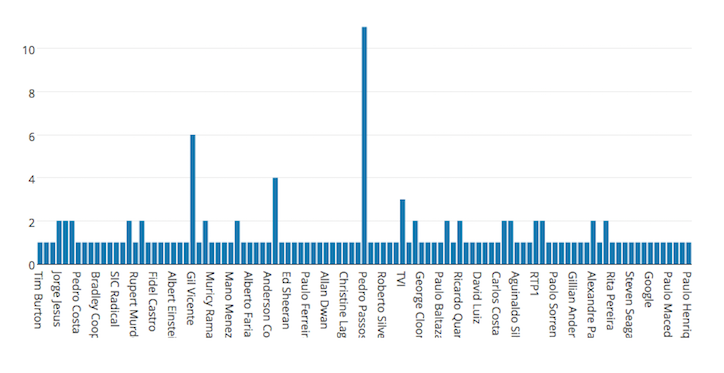
\includegraphics[width=0.9\textwidth]{images/day_one.png}
	\caption{Personalidades no dia 9 de maio de 2015}
\end{figure}

\begin{figure}[htbp]
  \centering
    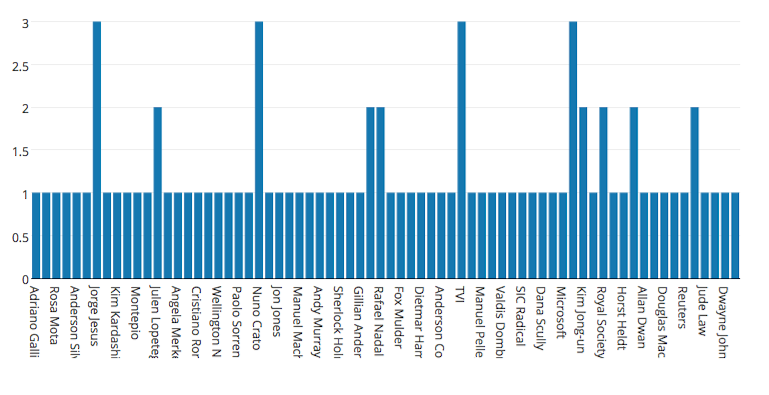
\includegraphics[width=0.9\textwidth]{images/day_two.png}
	\caption{Personalidades no dia 13 de maio de 2015}
\end{figure}

\begin{figure}[htbp]
    \centering
    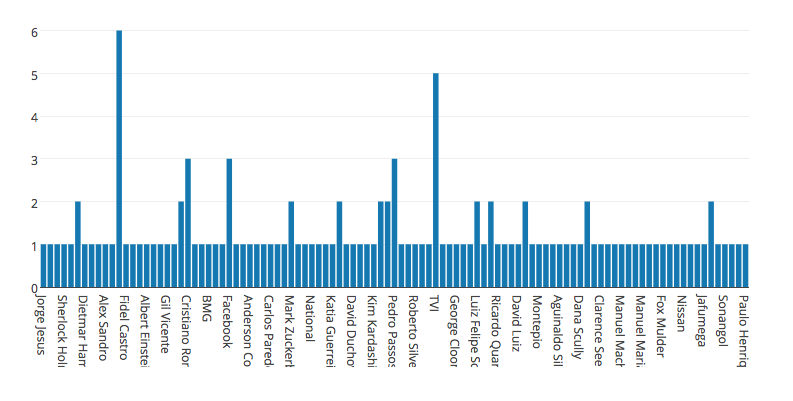
\includegraphics[width=1\textwidth]{images/search55.png} %trocar para imagem do dia 14 ou 15 de maio
    \caption{Personalidades no dia 14 de maio de 2015}
\end{figure}


\newpage
\section{Análise Crítica}
Com base nos exemplo que apresentamos nos anexos, verificamos que o nosso projecto podia sofrer bastantes melhorias na parte da recolha de entidades. Observa-se por exemplo, que na procura pela \textit{query} `morte` não foram encontradas quaisquer entidades nas quatro notícias devolvidas. Isto deve-se principalmente ao facto de a ferramenta \textit{nltk} estar preparada para a análise de texto na língua inglesa. Uma melhoria a fazer no futuro seria usar o módulo \textit{floresta} do \textit{nltk} para tentar obter melhores resultados na língua portuguesa. Contudo, com base nos gráficos apresentados na secção estatísticas achamos que os resultados são satisfatórios pois, mesmo assim são encontrados várias entidades portuguesas.

\section{Conclusão}
Após a realização deste projecto, concluímos que podíamos ter obtido melhores resultados em certas partes do projecto. A linguagem \textit{python} é adequada a este tipo de projectos pois tem disponível um grande conjunto de ferramentas que torna a extração e o processamento de informação um processo mais simples.
\section{Anexos} \label{anexos}
De referir que todos este exemplos são referentes às notícias extraídas no dia 13/05/2015.
\subsection{Procura e descoberta de entidades}
\begin{figure}[htbp]
  \centering
    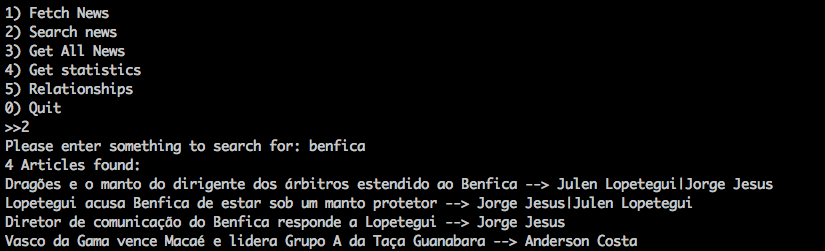
\includegraphics[width=0.9\textwidth]{images/search3.png}
	\caption{Procura pela query `benfica`}
\end{figure}

\begin{figure}[htbp]
  \centering
    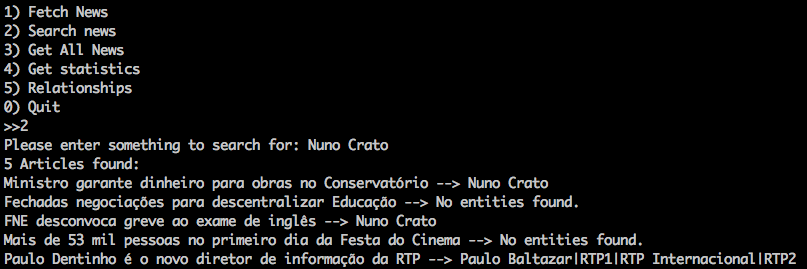
\includegraphics[width=0.9\textwidth]{images/search4.png}
	\caption{Procura pela query `Nuno Crato`}
\end{figure}

\begin{figure}[htbp]
  \centering
    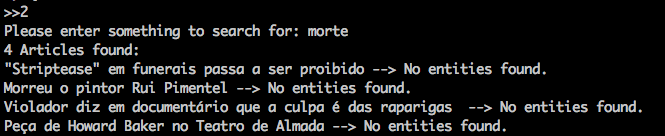
\includegraphics[width=0.7\textwidth]{images/search77.png}
	\caption{Procura pela query `morte`}
\end{figure}

\newpage
\subsection{Relações entre entidades}
\begin{figure}[htbp]
  \centering
    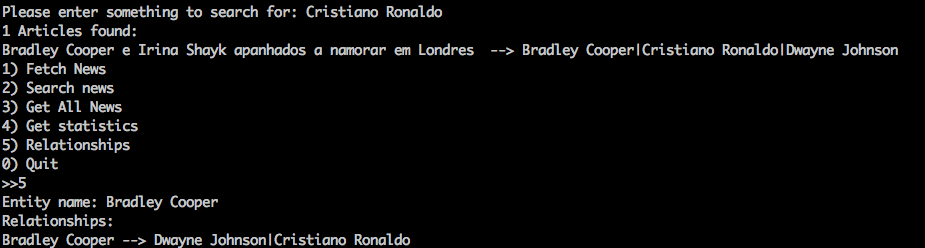
\includegraphics[width=0.9\textwidth]{images/search5.png}
	\caption{Procura por entidades relacionadas com Bradley Cooper}
\end{figure}

\subsection{Estatísticas}

\begin{figure}[htbp]
  \centering
    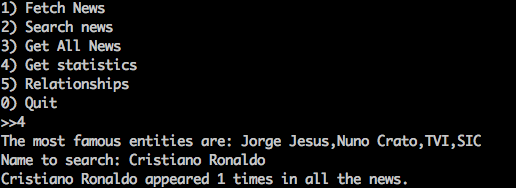
\includegraphics[width=0.5\textwidth]{images/search7.png}
	\caption{Estatísticas acerca de Cristiano Ronaldo}
\end{figure}
\end{document}